\section{Manual de uso de la skill}


\textbf{Requisitos}: disponer de un dispositivo de Alexa con pantalla rectangular (como un Amazon Echo Show), que tenga la skill instalada y conexión estable a Internet.

\vspace{0.5cm}

\textbf{Recomendaciones antes de jugar}: la cantidad recomendada de participantes, ya sea en modo por equipos o jugadores individuales, para una experiencia de juego divertida y fluida es mínimo 2 y máximo 5. 

También aconseja que haya una persona que actúe como supervisora, que puede ser la encargada de iniciar y configurar la partida, incluso de guardarla y finalizarla en caso de que deba dejarse a medias.

\vspace{0.5cm}

El primer paso es lanzar la skill, para lo que es necesario decir \textbf{\textit{<<Alexa, abre probando oca>>}}.

Alexa mostrará la pantalla de inicio (ver \autoref{fig:manual-1}) y dará un mensaje de bienvenida a los jugadores, con indicaciones básicas de cómo empezar el juego.

\begin{figure}[H]
	\centering
	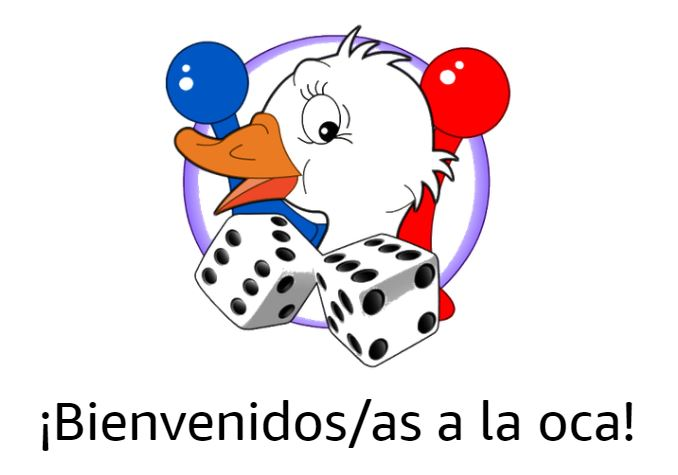
\includegraphics[width=0.6\textwidth]{imgs/interfaz-1.JPG}
	\caption{Pantalla de inicio de la skill del juego de la oca}
	\label{fig:manual-1}
\end{figure}

Para más información acerca del juego, se le puede pedir a Alexa que explique con más profundidad ciertos temas, diciendo: \textbf{\textit{<<Explícame [tema]>>}}. Los temas de ayuda disponibles son: 
\begin{enumerate}
	\item \textbf{Las reglas del juego}: hará una descripción general del juego y los objetivos a cumplir para ganar. Estos últimos son: llegar a la meta en primer lugar y/o conseguir la mayor cantidad de puntos a través de los minijuegos.
	\item \textbf{Las casillas}: ofrece una breve explicación de cada tipo de casilla. Consultar escenario C.
	\item \textbf{Los minijuegos}: menciona los minijuegos que hay y en qué consiste cada minijuego. Consultar escenario D.
	\item \textbf{Los comandos de voz}: comenta brevemente los comandos de voz que el usuario puede utilizar para interactuar con la skill. Consultar cuadro 34.
\end{enumerate}

Además, si en cualquier momento se intenta realizar una acción no válida o transcurre un determinado tiempo sin que Alexa reciba respuesta, se activará un mensaje de ayuda recordando el estado actual de la partida y cómo progresar adecuadamente a partir de ese punto.

\begin{table}[H]
	\centering
	\begin{tabular}{|c|p{8.5cm}|}
		\hline
		\rowcolor{lightgray}
		\textbf{Comando} & \textbf{Cuándo puede invocarse}\\
		\hline
		Abrir la skill & En cualquier momento, mientras no se haya iniciado la skill aún \\
		\hline
		Ayuda/Explicación de tema & En cualquier momento \\
		\hline
		Nueva partida & En cualquier momento, pero sobrescribe los últimos datos de partida guardados \\
		\hline
		Continuar partida & En cualquier momento, pero sobrescribe los datos de partida actuales \\
		\hline
		Guardar partida & Al inicio de cualquier turno, antes de tirar el dado \\
		\hline
		Cerrar la skill & En cualquier momento, con el riesgo de perder el progreso actual si no se ha guardado la partida \\
		\hline
		Tirar dado & Al inicio del turno de un participante o después de haber caído en una casilla de oca \\
		\hline
		Mover ficha & Después de un lanzamiento de dado \\
		\hline
	\end{tabular}
	\caption{Lista de comandos de voz y ámbito de uso}
	\label{tab:comandos-voz}
\end{table}

\textbf{Escenario A: Iniciar una nueva partida.}

Para comenzar una nueva partida, se debe decir \textbf{\textit{<<Nueva partida>>}}.

Alexa procederá a pedir de forma secuencial los datos necesarios para configurar la partida en proceso de creación, en el siguiente orden:
\begin{enumerate}
	\item \textbf{El modo de juego}: las dos opciones son <<por equipos>> o <<jugadores individuales>>. Este parámetro afectará a la forma en la que Alexa se refiere a los participantes (en singular o plural).
	\item \textbf{El número de participantes} (equipos o jugadores) que van a competir. Debe ser una cifra entera entre 1 y 5.
	\item \textbf{El nombre de cada participante}. Alexa dará indicaciones sobre cómo registrar un nombre y luego irá preguntado a cada participante, uno por uno. La sintaxis que hay que seguir para ello es: \textbf{\textit{<<Mi/Nuestro nombre es [nombre]>>}}.
\end{enumerate}

Una vez registrados todos los datos, Alexa hará un resumen general de la configuración de la partida, y mostrará por pantalla la información de todos los equipos/participantes del juego (ver \autoref{fig:manual-2}), tras lo cual se pasará al escenario C.

\begin{figure}[H]
	\centering
	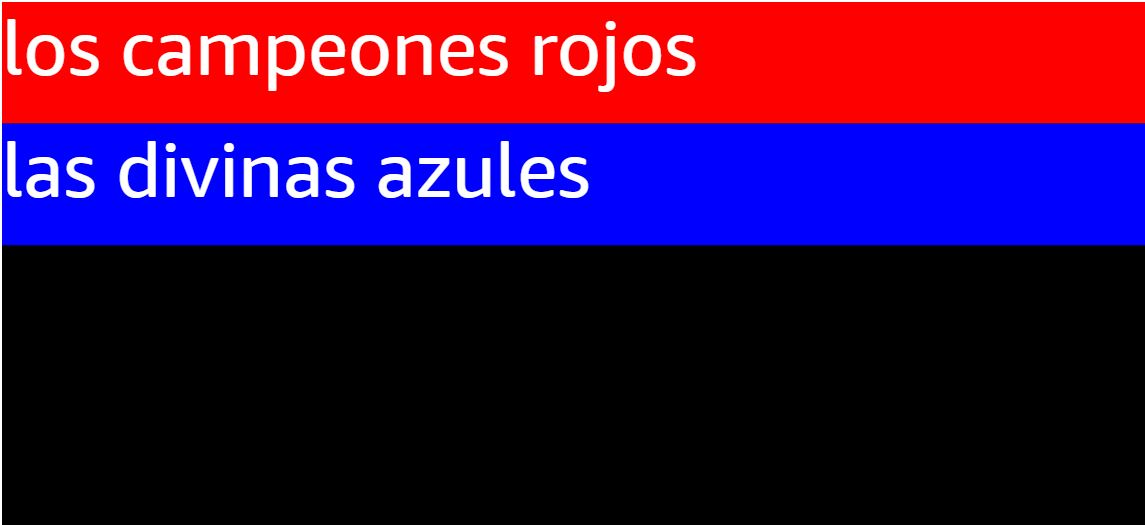
\includegraphics[width=0.6\textwidth]{imgs/interfaz-2.JPG}
	\caption{Pantalla de inicio de la skill del juego de la oca}
	\label{fig:manual-2}
\end{figure}

\textbf{Escenario B: Continuar con la partida anterior.}

Si se ha guardado anteriormente una partida, la próxima vez que se inicie una sesión de la skill se podrá retomar desde el punto en el que se dejó, mediante la instrucción \textbf{\textit{<<Continuar partida>>}}.

Esto permitirá cargar el estado de la partida desde la base de datos y continuar el juego a partir del último turno registrado, omitiendo entonces el Escenario A y pasando al C directamente.

\vspace{0.5cm}

\textbf{Escenario C: Jugar un turno.}

Durante la partida, Alexa anunciará el turno del equipo/participante actual. Cada turno se compone de dos fases clave: el lanzamiento de dado y el movimiento de su ficha.

Para tirar el dado, dicho participante o un integrante del equipo debe decir \textbf{\textit{<<Tirar dado>>}}, lo que llevará a mostrar la animación y el resultado del lanzamiento.

\begin{figure}[H]
	\centering
	
\includegraphics[width=0.6\textwidth]{imgs/interfaz-3.JPG}
	\caption{Pantalla de lanzamiento de dado con resultado 1}
	\label{fig:manual-3}
\end{figure}

Acto seguido, debe decir \textbf{\textit{<<Mover ficha>>}} para poder avanzar tantas posiciones como indique el dado. El juego lo colocará en la nueva casilla, que dependiendo de su tipo, puede implicar el final de dicho turno o el inicio de una nueva acción:
 \begin{itemize}
 	\item \textbf{Casilla normal}: se narra un evento concreto en función de la casilla en la que haya caído, que puede variar de unas veces a otras, y finaliza el turno.
 	\item \textbf{Casilla de oca}: se mueve a la siguiente casilla del mismo tipo y puede tirar de nuevo el dado. En el caso en el que haya caído en la oca anterior a la casilla de meta, se traslada a esta última y finaliza el juego.
 	\item \textbf{Casilla de puente}: solo existen dos de este tipo, y caer en una provoca el desplazamiento inevitable a la otra, tras lo cual finaliza el turno. 
 	\item \textbf{Casilla de penalización}: a su vez se distinguen cuatro tipos (pozo, laberinto, hotel y cárcel), entre los que puede variar el número de turnos que hay que esperar antes de poder avanzar de nuevo.
 	\item \textbf{Casilla de minijuego}: por lo general, implica que Alexa le haga una pregunta de untipo concreto para la posibilidad de ganar puntos si se acierta. Para un desglose de los tipos de juegos y respuestas aceptadas, consultar el escenario D.
 	\item \textbf{Casilla de meta}: se da la enhorabuena a los ganadores o ganadores (quienes hayan llegado antes a la meta y/o hayan logrado acumular más puntos con los minijuegos), y se da por finalizada la partida.
 \end{itemize}

Para guiar mejor a cada persona usuaria, se mostrará en la pantalla la casilla en la que ha caído, junto con sus datos de jugador/a, tras mover su ficha (ver \autoref{fig:manual-4}).
\begin{figure}[H]
	\centering
	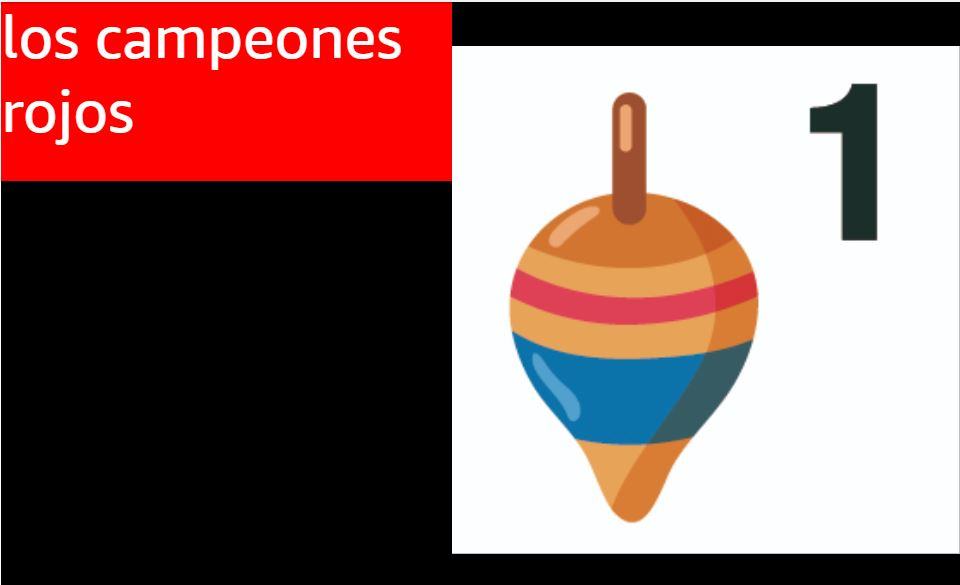
\includegraphics[width=0.6\textwidth]{imgs/interfaz-4.JPG}
	\caption{Pantalla al final del turno con los datos de la posición actual}
	\label{fig:manual-4}
\end{figure}

\textbf{Escenario D: Participar en un minijuego}

A este escenario se llega solo si se cae en una de las casilla de minijuego, por lo que la cantidad de puntos acumulados no solo depende de cuántas se acierten, sino también de la frecuencia en la que se caiga en ellas para aumentar la posibilidad de sumar puntos al marcador.

Dependiendo del tipo de casilla de minijuego que sea, se dan las siguientes situaciones:
\begin{itemize}
	\item \textbf{Verdadero o falso}: Alexa hace una pregunta de verdadero o falso. Si la respuesta es correcta, se añaden 10 puntos.
	\item \textbf{Adivina la cifra}: Alexa hace una pregunta cuya respuesta es un número. Si se acierta, se ganan 30 puntos, si no, la pregunta rebota al siguiente equipo/participante, y así sucesivamente hasta que alguien acierte o todos hayan dado respuestas incorrectas, entonces Alexa revelará la solución.
	\item \textbf{Conoce a tus compañeros}: Alexa formulará una pregunta acerca de uno de los compañeros, que se elige de manera aleatoria. El primero responde con lo que piense que es correcto, y será el propio sujeto de la pregunta el que tenga que confirmar si su respuesta es correcta o no. Si lo es, ambos ganan 15 puntos.
	\item \textbf{Recuerda la última casilla}: desafía la memoria a corto plazo, pues Alexa preguntará por el nombre de la última casilla en la que estuvo. Si es capaz de acordarse, ganará 25 puntos y si no, se revelará la solución.
	\item \textbf{Recuerda la fecha}: Alexa hace una pregunta cuya respuesta puede ser un día de la semana, mes o estación del año concreta, por la oportunidad de ganar 20 puntos. Para hallar la respuesta correcta, es necesario acordarse de la fecha actual, por lo que pone a prueba la noción del tiempo y memoria de la actualidad de quienes juegan.
\end{itemize}

Para entender mejor el tipo de respuestas esperadas en cada minijuego, se puede consultar la tabla siguiente.
\begin{table}[H]
	\centering
	\begin{tabular}{|c|p{7cm}|}
		\hline
		\rowcolor{lightgray}
		\textbf{Minijuego} & \textbf{Formato de respuesta esperada}\\
		\hline
		Trivial V/F & Verdadero o falso \\
		\hline
		Conoce a los participantes & Correcto/a o incorrecto/a \\
		\hline
		Adivina la fecha & Un número entero positivo \\
		\hline
		Recuerda la última casilla & El nombre de una casilla \\
		\hline
		Recuerda la fecha & El nombre de un día de la semana, mes o estación del año \\
		\hline
	\end{tabular}
	\caption{Tipos de respuestas del usuario a los minijuegos}
	\label{tab:respuestas-minijuegos}
\end{table}

\textbf{Escenario E: Terminar la partida}

Basta con decir \textbf{\textit{<<Cierra probando oca>>}} para cerrar la skill y por tanto finalizar la partida, sin embargo, esta acción borrará de manera permanente los datos de la partida actual a no ser que se hayan guardado previamente.


